\documentclass[xcolor=table,mathserif,9pt]{beamer}    % ,handout
% colortbl only defines \rowcolor for a single row. xcolor extends this to multiple rows.

\usetheme{Aachen}
\usepackage[english]{babel}
\usepackage[utf8]{inputenc}
%\usepackage{tikz-dependency}
%\usepackage{chronology}
\usepackage{array, booktabs}
\newcommand{\foo}{\makebox[0pt]{\textbullet}\hskip+0.5pt\vrule width 5pt\hspace{\labelsep}}
\usepackage{multirow}
\usepackage{textcomp}
\usepackage{media9}
\usepackage{csquotes}
\usepackage{amsmath}
\usepackage[]{algorithm2e}
\usepackage{lipsum}
\usepackage{multicol}
\usepackage{hyperref}
\setlength{\columnsep}{1cm}
%%%%%%%%%%%%%%%%%%%%%%%%%%%%%%%%%%%%%%%%%%%%%%%%%%%%%%%%%%%%%%%%%%%%%%
% tables
\usepackage{multirow,array,tabularx,rotating}
\usepackage{booktabs}
\usepackage{tabularx}

% math
\usepackage{amsmath,amsthm, amssymb, latexsym, xspace}
%\usepackage{bbold}
\usefonttheme[onlymath]{serif}
\boldmath


% misc
\usepackage{subfigure}
\usepackage{wasysym}
\usepackage{nameref}
\usepackage{xcolor}
\usepackage{romannum}
% declare the path(s) where your graphic files are
\graphicspath{{./nlu/}{./g2p/}{./smt/}}
% and their extensions so you won't have to specify these with
% every instance of \includegraphics
\DeclareGraphicsExtensions{.pdf,.jpeg,.png}


%figures
\usepackage{tikz}
\usepackage{minibox}
% change the graphic extentions
%\usepackage{ifpdf}
%\ifpdf
%  \DeclareGraphicsExtensions{.pdf,.png,.jpg}
%\else
%  \DeclareGraphicsExtensions{.eps}
%\fi

\usepackage[np,autolanguage]{numprint}
\nprounddigits{1}

% helpers
\newcommand{\argmin}{\operatornamewithlimits{argmin}}
\newcommand{\argmax}{\operatornamewithlimits{argmax}}
\newcommand{\sign}{\operatornamewithlimits{sign}}
\newcommand{\Eqn}{Equation}
\newcommand{\Eqns}{Equations}
\newcommand{\Fig}{Figure}
\newcommand{\Figs}{Figures}
\newcommand{\Tab}{Table}
\newcommand{\Sec}{Section}
\def\example{{\textit{}{e.g.}}\xspace}
\def\cad{{\textit{}{i.e.}}\xspace}
\def\etc{{\textit{etc.}}\xspace}
\def\apriori{{\textit{a priori}}\xspace}

\newcommand{\NetTalk}{NETtalk\xspace}
\newcommand{\Celex}{Celex\xspace}
\newcommand{\Pronlex}{Pronlex\xspace}
\newcommand{\gtp}{G2P}
\newcommand{\Seg}{\mathbb{S}}
\newcommand\BLEU{\textsc{Bleu}\xspace}
\newcommand\TER{\textsc{Ter}\xspace}
\newcommand\CTER{\textsc{CTer}\xspace}

\newcommand\AER{\textsc{Aer}\xspace}
\newcommand\SAER{\textsc{Saer}\xspace}
\newcommand{\GIZA}{{GIZA\nolinebreak[4]\hspace{-.025em}\raisebox{.2ex}{\small\bf++}}\xspace}

\newcommand{\todo}[1]{\colorbox{yellow}{#1}\xspace}
\newcommand{\CITE}{\colorbox{yellow}{CITE}\xspace}
\newcommand{\REF}{\colorbox{yellow}{REF}\xspace}
\newcommand{\EQ}{\colorbox{yellow}{REF}\xspace}
\newcommand{\NUMBER}{\colorbox{yellow}{NUMBER}\xspace}
\newcommand{\Align}{\mathbb{A}}
%\renewcommand{\emph}[1]{\textcolor{i6blue}{#1}}


\newcommand{\aind}[1]{\hspace*{#1ex}}
\newcommand{\gray}[1]{\textcolor{gray}{#1}}

\newcommand*{\sumw}{\ensuremath{\operatornamewithlimits{sum}}\xspace}
\newcommand*{\nbest}{\ensuremath{\operatornamewithlimits{nbest}}\xspace}

% Define box and box title style
\usepackage{tikz}
\usetikzlibrary{shapes,positioning,fit}
\tikzstyle{bubble} = [ draw=blue, rectangle, rounded corners, inner sep=3pt, inner ysep=
10 pt]
\tikzstyle{fancytitle} =[fill=white, text=black]
\newenvironment{bubble}[3]{%
  \begin{tikzpicture}[transform shape, baseline=-0.5 cm]
  \def\bubbletitle{#1}%
  \node [bubble] (box)\bgroup
  \begin{minipage}[t][#3]{#2}%
}{%
  \end{minipage}%
  \egroup;
  \node[fancytitle] at (box.north) {\bubbletitle};
  \end{tikzpicture}%
}

\newenvironment{bubble*}[2]{%
  \begin{tikzpicture}[transform shape]
  \node [bubble] (box)\bgroup
  \begin{minipage}[t][#2]{#1}%
}{%
  \end{minipage}%
  \egroup;
  \end{tikzpicture}%
}

% CUSTOM STUFF %%%%%%%%%%%%%%%%%
%\usepackage{neuralnetworks}


% Rounding commands
\def\roundpositionii{1}
\newcommand{\rdmii}[1]{\edef\rounded{0}\FPeval\rounded{round(#1,\roundpositionii)}\rounded}
\def\roundpositioni{1}
\newcommand{\rdmi}[1]{\edef\rounded{0}\FPeval\rounded{round(#1,\roundpositioni)}\rounded}
\def\roundposition{0}
\newcommand{\rdm}[1]{\edef\rounded{0}\FPeval\rounded{round(#1,\roundposition)}\rounded}

\npstyleenglish

\def\roundposition{1}
\def\roundpositiont{3}
\edef\rounded{0}
\newcommand{\rd}[1]{\ifthenelse{\equal{#1}{--}}{--}{\edef\rounded{0}\FPeval\rounded{round(#1,\roundposition)}\rounded}}
\newcommand{\rdmt}[1]{\edef\rounded{0}\FPeval\rounded{round(#1,\roundpositiont)}\rounded}
\newcommand{\rp}[1]{%
  \FPset{\per}{#1}%
  %\FPmul{\per}{\per}{100}%
  \FPround{\per}{\per}{1}%
  \numprint{\per}%
}%


\setbeamercovered{transparent}

\DeclareMathOperator*{\sigmoid}{sigmoid}

\newcommand\T{\rule{0pt}{2.2ex}}       % Top strut
\usepackage{etoolbox}
\pretocmd{\section}{\addtocontents{toc}{\vspace{-20pt}}}{}{}

%Table stuff
\newcommand{\tablesize}{}
\newcommand{\abovetable}{\vspace{0.6cm}}
\newcommand{\belowtable}{\vspace{0.13cm}}


% Get fond size for system combination picture right
\usepackage{fix-cm}    
\makeatletter
\newcommand\SyscomFontSize{\@setfontsize\small{6}{60}}
\makeatother   

%%%%%%%%%%%%%%%%%%%%%%%%%%%%%%%%%

\newcommand{\backupbegin}{
   \newcounter{finalframe}
   \setcounter{finalframe}{\value{framenumber}}
}
\newcommand{\backupend}{
   \setcounter{framenumber}{\value{finalframe}}
}

\newcommand{\stoptocwriting}{%
  \addtocontents{toc}{\protect\setcounter{tocdepth}{-5}}}
\newcommand{\resumetocwriting}{%
  \addtocontents{toc}{\protect\setcounter{tocdepth}{2}}}

%%%%%%%%%%%%%%%%%%%%%%%%%%%%%%%%%%%%%%%%%%%%%%%%%%%%%%%%%%%%%%%%%%%%%%  
%%%%%%%%%%%%%%%%%%%%%%%%%%%%%%%%%%%%%%%%%%%%%%%%%%%%%%%%%%%%%%%%%%%%%%

\renewcommand*{\email}{\url{patrick.platen@rwth-aachen.de}}  
% all email address(es) of the authors (used for \TitlePage)

\title[Seminar]{Artificial Neural Network Supported Source Separation}
%\subtitle{Presentation Subtitle} % (optional)
%\setbeamertemplate{section in toc}[sections numbered] 
%\setbeamertemplate{subsection in toc}[subsections numbered] 
\setbeamertemplate{navigation symbols}{} %disable {, dotted}navigation bar

%% author and in []: shortauthorChange the scale of beamer from 3.5 to 1
\author[Patrick von Platen]{Patrick von Platen}
% - Use the \inst{?} command only if the author7s have different
%   affiliation.
\institute[RWTH Aachen University] % (optional, but mostly needed)
{
%  \inst{1}%
  \strut Human Language Technology and Pattern Recognition\\
  \strut Computer Science Department, RWTH Aachen University %\\
  %\strut {\tt lehnen@cs.rwth-aachen.de}
}
% - Use the \inst command only if there are several affiliations.
% - Keep it simple, no one is interested in your street address.

\date[19/6/2018]{June 19th, 2018}

%%%%%%%%%%%%%%%%%%%%%%%%%%%%%%%%%%%%%%%%%%%%%%%%%%%%%%%%%%%%%%%%%%%%%%shit
% will be set into the PDF document summary
\hypersetup{
  pdftitle={\inserttitle}, 
  pdfauthor={\insertauthor}, 
  bookmarksdepth=subsubsection,  
  % enable automatic page transitions: for endless loop edit in
  % acrobat reader -> preferences -> full screen -> after every X
  % seconds and after last page
  %pdfpageduration = 2, 
  % pdfpagetransition = {Glitter /Di 315 /D 5}  
  % pdfpagetransition = {Box /M /O /D 1},
} 
%%%%%%%%%%%%%%%%%%%%%%%%%%%%%%%%%%%%%%%%%%%%%%%%%%%%%%%%%%%%%%%%%%%%%%
%%%%%%%%%%%%%%%%%%%%%%%%%%%%%%%%%%%%%%%%%%%%%%%%%%%%%%%%%%%%%%%%%%%%%%

%%%%%%%%%%%%%%%%%%%%%%%%%%%%%%%%%%%%%%%%%%%%%%%%%%%%%%%%%%%%%%%%%%%%%%
%%%%%%%%%%%%%%%%%%%%%%%%%%%%%%%%%%%%%%%%%%%%%%%%%%%%%%%%%%%%%%%%%%%%%%
\begin{document}

%%%%%%%%%%%%%%%%%%%%%%%%%%%%%%%%%%%%%%%%%%%%%%%%%%%%%%%%%%%%%%%%%%%%%%
\begin{frame}[label=titlepage]
  \titlepage
\end{frame}

\begin{frame}
	\frametitle{Outline}
	\tableofcontents
        %\tableofcontents[currentsection, subsectionstyle=show/show/hide]
\end{frame}


%%%%%%%%%%%%%%%%%%%%%%%%%%%%%%%%%%%%%%%%%%%%%%%%%%%%%%%%%%%%%%%%%%%%%%


\section{Literature}%
\label{sec:literature}


\begin{frame}{Literature}
\begin{description}
\item [Z. Chen:] Single Channel auditory source separation with neural network. {\em thesis 2017}.
  \begin{itemize}
  \item Output permutation problem  
  \item Output dimension problem 
  \item Deep clustering
  \end{itemize}
\item [Yi Luo, Nima Mesgarani:] TasNet: time-domain audio separation network for real-time, single-channel speech separation {\em TasNet 2017}.
  \begin{itemize}
  \item TasNet 
  \end{itemize}
\item [M. Kolbæk and D. Yu and Z. H. Tan and J. Jensen: ]Multitalker Speech Separation With Utterance-Level Permutation Invariant Training of Deep Recurrent Neural Networks {\em pivT 2017}.
  \begin{itemize}
  \item Permutation invariant training 
  \end{itemize}
\item [Bach, Francis R. and Jordan, Michael I.: ]Learning Spectral Clustering, With Application To Speech Separation {\em SpectralClustering 2006}
\begin{itemize}
	\item Spectral Clustering
\end{itemize}
\end{description}
\end{frame}

\section{Introduction}%
\label{sec:introduction}
\begin{frame}{Source Separation}

\begin{center}
	\begin{figure}
	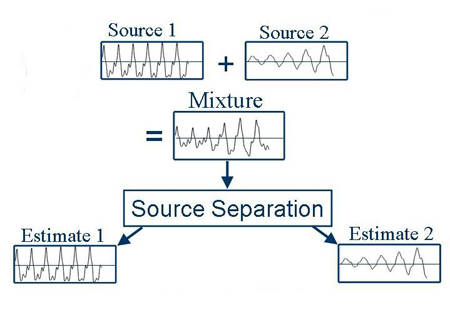
\includegraphics[width=.6\textwidth]{images/separation_example.jpg}
	\end{figure}
\end{center}

\end{frame}

\begin{frame}{History and Applications}

\begin{itemize}
	\setlength\itemsep{1em}
	\item History
	\begin{itemize}
		\item Cocktail Party Problem - first definition of source separation problem \cite{Cherry:1953} 
		\item Auditory Scene Analysis - first method for source separation \cite{bregman} 
		\item Spectral Clustering \cite{Bach:2006} 
		\item Deep Neural Networks for Speech Separation \cite{SpeechSepDeepLearning:2015} 
		\item Deep Clustering \cite{DeepClustering2016}
		\item TasNet \cite{TasNet2017}
	\end{itemize}
	
	\item Applications
	\begin{itemize}
		\item Automatic meeting transcription 
		\item Virtual assistant
		\item Automatic subtitling of music/video
	\end{itemize}
\end{itemize}

\end{frame}

\section{Definition}%
\label{sec:definition}
\begin{frame}{Definition}

\begin{itemize}
	\setlength\itemsep{1em}
	\item Formal definition: Single-channel blind source separation
	\begin{itemize}
		\item No spatial information $\to$  ``Single-channel''
		\item No information about sources in advance $\to$ ``Blind''
	\end{itemize}
	\item Mathematical definition
	\begin{itemize}
		\item Sources: $c = 1,...,C$
		\item Discrete time stepts: $t = 1,...,T$
		\item c-th source signal: $x_c(t)$
		\item Mixture: $X(t) = \sum_{c=1}^{C} x_c(t)$
		\item Goal: Recover $\{x_1(t),...,x_c(t)\}$ from $X(t)$
	\end{itemize}
\end{itemize}

\end{frame}

\section{Mathematical Basics}%
\label{sec:mathematical_basics}
\begin{frame}{Short time fourier transform \cite{664179}}

\begin{itemize}
	\setlength\itemsep{1em}
	\item Fourier transform 
	\begin{itemize}
		\item $S(f) = \int_{\mathbb{R}}X(t)e^{-2{\pi}jft}dt$
		\item Inverse Fourier transform: $X(t) = \int_{\mathbb{R}}S(f)e^{2{\pi}jft}df$
		\item Signal $X(t)$ can be decomposed to sum of weighted ``base frequencies''
		\item Fourier transform can be viewed as ``special convolution'' operation
	\end{itemize}
	\item Short time fourier transform
	\begin{itemize}
		\item Short time fourier transform: $S(f,t) = \int_{\mathbb{R}}X(\tau)w(\tau - t)e^{-2{\pi}jft}dt$ (called (f,t) bin in the following)
		\item Uncertainty in signal processing: Time localization vs. frequency precision \cite{DBLP:journals/corr/Nam13}
		\item Window function $w(\tau) = 0: \tau \not \in \left[-a, a \right]$ defines width of (f,t) bins 
	\end{itemize}
\end{itemize}

\end{frame}

\begin{frame}{Spectrogram}

\begin{itemize}
	\item Shows the result of short time fourier transform graphically
	\item Answers the question: \emph{Which frequencies are used at what time?}
\end{itemize}

\begin{center}
	\begin{figure}
		\includegraphics[width=.8\textwidth]{images/spectogram.png}
	\end{figure}
\end{center}

\end{frame}

\begin{frame}{Embedding}

	\begin{itemize}
		\item Structure-preserving, injective mapping $f: A \to B$
		\item $B$ is normed space: $d(b_1,b_2) \in \mathbb{R}, \forall b_1,b_2 \in B$
		\item Example is \emph{word2vec}: 
			\begin{itemize}
				\item ``house'' $\to \left[1, 8, -8, 4, 5, 3, 29, -34\right]^{T}$
				\item ``car'' $\to \left[8,9, -8, 8, 5, 5, -34, -25\right]^{T}$
				\item Using euclidean distance norm: $d(f(\text{``house''}),f(\text{``car''})) = 64.19$ 
			\end{itemize}
		\item Mapping $f: A \to B$ can be modelled using a neural network (see Deep Clustering)
	\end{itemize}



\end{frame}

\section{Spectral Clustering}%
\label{sec:spectral_clustering}

\begin{frame}{Spectral Clustering}
\begin{itemize}
	\item Consider dataset $D$ with $p$ datapoints: $D \in \mathbb{R}^p$.
	\item Similarity matrix $W \in \mathbb{R}^{p \times p}$ derived from $D$
\end{itemize}
\vspace{10mm}
\begin{algorithm}[H]
	\RestyleAlgo{boxruled}
	\LinesNumbered
	\emph{\textbf{Input: }} $(W, r)$ \\
	\emph{\textbf{Algorithm: }}
	\begin{itemize}
		\item Compute first $r$ eigenvectors $H: (h_1,... ,h_r) \in \mathbb{R}^{p \times r}$ of $W$ 
		\item Transpose $H$ to $O = H^T: (o_1,... ,o_p) \in \mathbb{R}^{r \times p}$ 
		\item Initialise clusters $Z$ and perform K-means \cite{Steinhaus56} using $(o_1,... ,o_p)$ 
	\end{itemize}
	\emph{\textbf{Output: }}$\textbf{Z} = (Z_1, Z_2, ..., Z_r)$
\end{algorithm}
\end{frame}

\begin{frame}{Spectral Clustering for Source Separation \cite{Bach:2006}}
	
How to derive similarity matrix from mixed signal: \emph{$X(t) \to W$}?
\vspace{10mm}
\begin{enumerate}
	\item Short time fourier transform: $X(t) \to (f,t)$ bins
	\item Apply handcrafted features: \emph{Energy, continuity, common fate cues, pitch estimation, timbre}: $(f,t) \text{ bins} \to (s_{k,1}, ...,s_{k,n}): n = F \times T$ for feature $k$ with $F$ and $T$ being amount of frequency and time bins.
	\item Create similarity matrix for every feature $k$ with $W_k(i,j) = f_k(s_{k,i},s_{k,j})$
	\item ``Put together'' similarity matrixes using $\odot$ and a  weight vector $\alpha$: $W = W_1^{\alpha_1} \odot ... \odot W_k^{\alpha_k} \odot ...$ 
	\item Apply spectral clustering algorithm 
\end{enumerate}
\vspace{10mm}

\begin{itemize}
	\item $\alpha$ is trained using labeled data $\to$ \emph{Linear regression}
\end{itemize}


\end{frame}

\section{Problems with Deep Learning}%
\label{sec:problems_with_deep_learning}
\begin{frame}{Output Dimension Problem \cite{SingleChannelSourceSeparation}}

\begin{itemize}
	\item size(output layer) = \textbf{\#sources} $\times$ size(input layer)
\end{itemize}

\begin{figure}[htpb]
	\centering
	\includegraphics[width=0.8\linewidth]{images/outputDimProblem.png}
	\caption{Output dimension problem}
\end{figure}

\end{frame}

\begin{frame}{Output Permutation Problem \cite{SingleChannelSourceSeparation}}
	\begin{itemize}
		\item Label of speaker has to be assigned to ``matching'' part of output layer
	\end{itemize}

	\begin{figure}[htpb]
		\centering
		\includegraphics[width=0.8\linewidth]{images/permutationDimProblem.png}
		\caption{Output permutation problem}
	\end{figure}

\end{frame}

\section{Deep Clustering}%
\label{sec:deep_clustering}
\begin{frame}{Deep Clustering \cite{SingleChannelSourceSeparation}, \cite{BasicDeepClustering:2016}}

\begin{enumerate}
	\item $X(t) \to (f,t)$ bins
	\item $(f,t) \text{ bin } \to \text{ embedding }$ (encoding) via neural network
	\item Encodings are clustered via K-means
\end{enumerate}

\begin{figure}[htpb]
	\centering
	\includegraphics[width=0.8\linewidth]{images/deepClustering.png}
	\caption{Deep clustering}
\end{figure}

\end{frame}

\begin{frame}{Deep Clustering - Encoding}

 \begin{itemize}
	 \item $(f,t)$ bins are transformed to 
		 $s = (s_1, ..., s_n)$  with $n = T \times F$
	 \item Neural network: \emph{$f_{\theta}(s) = V$} with: 
		\begin{itemize}
			\item $\theta$ being the parameters of the neural network
			\item $|s|$ size of input layer
			\item $V \in \mathbb{R}^{n \times K}$ being the embedding
			\item Neural network has $K$ parallel output layers of size $n$
		        \item $v_1, ..., v_n$ with \emph{$|v_i|^2 = 1$} normalized rows of $V$
			      each representing an embedding of $(f,t)$ bin 
			\item $v_{i,1}, ..., v_{i,k}$ analog to $k$ handcrafted 
			      features applied to $s_i$
		\end{itemize}
 \end{itemize}
\end{frame}

\begin{frame}{Deep Clustering - Clustering}

\begin{itemize}
	\item $v_1, ..., v_n$ are clustered using \emph{K-means loss function} 
	\item \emph{$Y^* = \text{argmin}_{Y} {V - YUF}$}
		\begin{itemize}
			\item $Y = (y_1,... ,y_n)^T \in \mathbb{R}^{n \times C}$
			\item $ y_i \in \mathbb{R}^{C}$. $y_i$ is cluster assignment of i-th (f,t) bin 
			\item Normalizer $U = (Y^TY)^{-1} \in \mathbb{R}^{C \times C}$
			\item Accumalator $F = Y^TV \in \mathbb{R}^{C \times K}$
		\end{itemize}
	\item Create masks \emph{$S_i = Y^*(c) \odot s$} with $\hat{Y}$ being one-hot encoded.
	\item Output dimension problem is solved 
\end{itemize}
	
\end{frame}

\begin{frame}{Deep Clustering - Training}
	
	\textbf{Minimize cost function $C(\theta)$}
	\begin{itemize}
		\item $C(\theta) = |VV^T - \hat{Y}\hat{Y}^T|_F^2$
		\item Frobenius norm: $|E|^2_F = \sum_{i,j} E(i,j)^2$ 
		\item $VV^T \in \mathbb{R}^{n \times n}$ estimated affinity matrix 
		\item $\hat{Y}\hat{Y}^T \in \mathbb{R}^{n \times n}$ labeled affinity matrix
		\item Intuitive presentation: 
			\begin{align*}
				C(\theta) &= \sum_{i,j}(v_i^T v_j - \hat{y_i}^T \hat{y_j})^2 \\
					... \\
					   &= \emph{\sum_{i,j; \hat{y_i} = \hat{y_j}} |v_i - v_j|^2 + \sum_{i,j} (v_i^T v_j)^2 - N}
			\end{align*}
		\item Permutation invariant: $VV^T(i,j) = VV^T(j,i)$
	\end{itemize}
		
\end{frame}

\begin{frame}{Deep Clustering - Training}
	
\begin{figure}[htpb]
	\centering
	\includegraphics[width=0.95\linewidth]{images/dcExample.png}
	\caption{reprinted from Lensson}
\end{figure}

\end{frame}

\section{TasNet}%
\label{sec:tasnet}
\begin{frame}{TasNet \cite{TasNet2017}}

\begin{figure}[htpb]
	\centering
	\includegraphics[width=0.9\linewidth]{images/tasNetAll.png}
	\caption{TasNet}
\end{figure}
\vspace{10mm}
\begin{itemize}
	\item Neural network is applied to \emph{chunks of raw signal}
\end{itemize}

\end{frame}

\begin{frame}{Encoding - TasNet}

\begin{minipage}[t]{0.48\linewidth}
	\begin{figure}[htpb]
		\centering
		\includegraphics[width=0.9\linewidth]{images/tasNetEncoding.png}
	\end{figure}
\end{minipage}%
\hfill%
\begin{minipage}[t]{0.48\linewidth}
	\begin{itemize}
		\item Mixed signal $X$ is divided into $K$ chunks $X_k$ 
		\item Gated convolution is applied to $X_k$: 
			\emph{$w_k = \text{ReLu}(X_k * L_{\text{base}}) \odot \text{Sigmoid}(X_k * L_{\text{gate}})$} with layer weights $L_{\text{base}}$ and $L_{\text{gate}}$
	\end{itemize}
	\vspace{5mm}
	\begin{itemize}
		\item Signal as sum of base functions: $X = wB$
		\item Weight vector $w \in \mathbb{R}^{N}$ with $N$ = 
		      dimension of output layer
		\item Basis functions $B = (b_1, ...,b_n)$ 
		\item $w$ gives magnitude of basis functions $B$
		\item Gated convolution is \emph{$w = B^{-1}x$}
	\end{itemize}
\end{minipage}	



\end{frame}

\begin{frame}{Separation}

\begin{minipage}[t]{0.48\linewidth}
	\begin{figure}[htpb]
		\centering
		\includegraphics[width=0.7\linewidth]{images/tasNetSeparation.png}
	\end{figure}
\end{minipage}%
\hfill%
\begin{minipage}[t]{0.48\linewidth}
	\hfill
	\begin{itemize}
		\item weights $w$ are normalized $w \to \hat{w} = \frac{g}{\sigma} \odot (w - \mu) + b$ 
		\item $\sigma$ and $\mu$ are \emph{variance} and \emph{mean}
		\item $g,b$ are gain and bias vector
		\item Deep recurrent neural network $f_{\theta_s}$ outputs weight masks for every
			speaker: $M = (m_1, ...,m_k)  = f_{\theta_s}(w)$
		\item Size(outputLayer) = Size(inputLayer) $\times$ $\#$Speakers
		\item Output dimension problem is not solved in TasNet
	\end{itemize}
\end{minipage}	

\end{frame}

\begin{frame}{Decoding - TasNet}

\begin{minipage}[t]{0.48\linewidth}
	\begin{figure}[htpb]
		\centering
		\includegraphics[width=0.8\linewidth]{images/tasNetDecoding.png}
	\end{figure}
\end{minipage}%
\hfill%
\begin{minipage}[t]{0.48\linewidth}
	\hfill
	\begin{itemize}
		\item $w_i = m_i \odot w$: separate weight vectors
		\item Deconvolution operation to get raw signal: $X_i = w_iB$ 
		\item $X_i = \text{deconv}_{\theta_d}(w_i)$ with $\theta_d$
			parameters of deconvolutional layer 
		\item Chunks of signal $X_k$ can individually be separated $\to$ 
		      very \emph{low latency time} when decoding
	\end{itemize}
\end{minipage}	

\end{frame}

\begin{frame}{Permutation Invariant Training \cite{7979557}}
\begin{minipage}[t]{0.48\linewidth}
\hfill
\begin{figure}[htpb]
	\centering
	\includegraphics[width=0.9\linewidth]{../images/piv_train.png}
	\caption{Permutation invariant training}
\end{figure}
\end{minipage}
\hfill
\begin{minipage}[t]{0.48\linewidth}
\begin{itemize}
	\item source-to-noise ration $SNR$ \cite{AudioSpeechLanguageProcessing} is used as training criterion
	\item $\text{SNR}_i  = 10\log_{10}\frac{|s_{i}|^2}{|e_{i}|^2}$
	\begin{itemize}
		\item $s_{i} = \frac{X_i^TX_i^{*}X_i^{*}}{|X_i^{*}|^2}$
		\item $e_i = X_i - s_i$
	\end{itemize}
	\item \emph{$L(\theta_{all}) = \sum_{i=1}^C \text{SNR}_i$}
	\item Need ``correct'' permutation of labels  
	\item At every training step, mean-squared error of weight masks for correct assignment
	\item $ \theta^{*} = \text{argmin}_{\theta \in \mathcal{P}} \sum_{i=1}^{c} |m_i \odot w - w_i^{*}(\theta(i))|^2$ 
	\item $w_i^{*}$ from convolutional layer applied to $X_i^{*}$
\end{itemize}
\end{minipage}

\end{frame}

\section{Comparison and Results}%
\label{sec:results}
\begin{frame}{Comparison and Results}

\begin{table}
\centering
\begin{tabular}{|c|c|c|}
	\hline
	 & \emph{TasNet} & \emph{Deep Clustering}  \\
	\hline
	 Pro      & low latency time & no dimension output problem \\
	 $SNR$   & 10.8   & 10.8  \\
	\hline
\end{tabular}
\end{table}

\vspace{10mm}
\begin{itemize}
	\item Results taken on two-speaker WSJ0-2mix dataset \cite{TasNet2017}
	\item WSJO-2mix dataset consists of 7193 sentences from 42 female and 42 male         speakers amounting to 12.2 hours of speech
\end{itemize}
\end{frame}

\begin{frame}{Conclusion}

\begin{itemize}
	\item Methods improved greatly over the last 4 years
	\item More and more end-to-end approaches are succesfully applied 
	\item State-of-the-art: \emph{End-to-End Speech Separation with Unfolded Iterative Phase Reconstruction} yielding SNR: 12.8 on WSJ0-2mix \cite{2018arXiv180410204W}
\end{itemize}

\end{frame}

%%%%%%%%%%%%%%%%%%%%%%%%%%%%%%%%%%%%%%%%%%%%%%%%%%%%%%%%%%%%%%%%%%%%%%%%%%%%%%%%

\begin{frame}[label=finalSlide]
  \label{LastPage}%
  \begin{center}
    \vfill
    {\Large
    \textcolor{i6bluedark}{Thank you for your attention}
    }
%     \vfill
%     \inserttitle
    \vfill
    {\insertauthor}

    \vspace{10mm}
    \url{patrick.platen@rwth-aachen.de}
  \end{center}
\end{frame}

\nocite{*}

\stoptocwriting
\section{Appendix}
\resumetocwriting

%\backupbegin


%%%%%%%%%%%%%%%%%%%%%%%%%%%%%%%%%%%%%%%%%%%%%%%%%%%%%%%%%%%%%%%%%%%%%%%%%%%%%%%%
\section*{Appendix}



%%%%%%%%%%%%%%%%%%%%%%%%%%%%%%%%%%%%%%%%%%%%%%%%%%%%%%%%%%%%%

\begin{frame}[allowframebreaks]
  \centerline{Reference}
 %\bibliographystyle{ieeetr}
 \bibliographystyle{i6bibstyle}
 \bibliography{references}
\end{frame}

%\backupend

\end{document}
